\documentclass{standalone}
\usepackage{tikz}
\usepackage{ctex,siunitx}
\setCJKmainfont{Noto Serif CJK SC}
\usepackage{tkz-euclide}
\usepackage{amsmath}
\usepackage{wasysym}
\usetikzlibrary{patterns, calc}
\usetikzlibrary {decorations.pathmorphing, decorations.pathreplacing, decorations.shapes,}
\begin{document}
\small
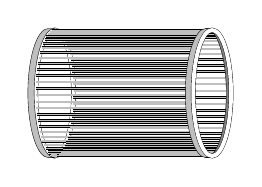
\begin{tikzpicture}[>=latex,scale=0.8]
  % \useasboundingbox(0.9,0)rectangle(5.1,5);
  \draw[double,double distance=0.5mm,line width=0.05mm](0,0)ellipse(0.3 and 1.0);
  \draw[line width=0.05mm,fill=lightgray](0,1.025)--(-0.1,1.025)arc(90:270:0.325 and 1.025)--(0,-1.025)arc(270:90:0.325 and 1.025)--cycle;
  \foreach \x in {0,6,...,360}
  {
    \draw[double=lightgray,line width=0.05mm]({0.3*cos(\x+2)},{sin(\x+2)})--++(2.5,0);
  }
  \draw[line width=0.05mm,fill=lightgray](2.5,1.025)--(2.4,1.025)arc(90:270:0.325 and 1.025)--(2.5,-1.025)arc(270:90:0.325 and 1.025)--cycle;
  \draw[line width=0.05mm,fill=gray](2.5,1.025)--(2.4,1.025)arc(90:-90:0.325 and 1.025)--(2.5,-1.025)arc(-90:90:0.325 and 1.025)--cycle;
  \draw[double,double distance=0.5mm,line width=0.05mm](2.5,0)ellipse(0.3 and 1.0);
\end{tikzpicture}
\end{document}